\section{Problem statement}
\label{sec:intro:problem}

More than 2.5 quintillion bytes of data are produced daily as the field of data
analysis continues to grow. ``Statistical thinking and methodology'' has become
the framework for disciplines such as education, agriculture, economics,
biology, medicine, astronomy, geology, and physics~\cite{efron1986}, but there
is still a lack of accountability and consistency in the field. What is striking
in the current practice of data analysis is the lack of progress on this
particular subject beyond the development of numerical methods. The rapid
increase in computing resources has led to the proliferation of high-dimensional
data sets, which require much more work to efficiently understand patterns in 
the data and verify numerical estimators. In fact, the ``physical limitations 
of display devices and our [human's] visual system prevent the direct display 
and instantaneous recognition of structures with higher dimensions than 
\textit{two or three}''~\cite{lius2016} (emphasis mine). 
One solution is to manually plot all variables against each other, but this 
becomes computationally tedious and unfeasible to sort through when there are 
even a few hundred variables. This problem gets even more complicated when 
considering \textit{interaction terms} (various transformations or combinations 
of explanatory variables). As such, the problem with current visual 
high-dimensional data analysis is that there are too many
potential plots to sort through manually, which increase quadratically with the 
number of variables. Furthermore, although methods for dimension reduction have 
been developed~\cite{lius2016}, it is still unclear how the analyst can easily 
check the resulting model to ensure that the variables which were culled in the 
dimension reduction process are actually undesirable.

In computer science, a framework for ``clean code'' has been extensively
documented and is the accepted industry standard for writing, interacting with,
and thinking about code. But in empirical data analysis with large data sets,
analysts blindly depend on estimators and hypothesis tests to explore the data
and have no justification of their analysis aside from asymptotic, mathematical
guarantees. Furthermore, since each estimator inherently performs well or poorly
under different settings, data analysts are unable to differentiate between the
properties intrinsic to the data set and the spurious properties the estimators
added. Little, a Professor of Biostatics at the University of Michigan, notes
that ``developing good statistical solutions to real applied problems, based on
good science rather than `cookbookery,' is far from easy''~\cite{little2013}.
This lack of agreement and ``cookbook'' mentality of data analysis has
far-reaching consequences. It is simple to run the data through a list of many
estimators and cherry-pick the most ``interesting'' result. Similarly, an
analyst can remove ``undesirable'' data points without justification or 
unknowingly fit egregiously incorrect models. Regardless of whether these 
situations are performed maliciously or with good intentions, the art of data 
analysis is unclear without standards. The lack of clear-cut guidelines makes 
it difficult for analysts to discern the ``truth'' from the data and avoid the 
aforementioned pitfalls while simultaneously making it difficult for consumers 
of the resulting analysis to evaluate how trustworthy it is. These difficulties 
arise due to the difficulty in visualizing high-dimensional data. Plotting is 
one of the most consistent and universally interpretable ``sanity checks'' for 
numerical results; without it, effective and accountable analysis is difficult 
to achieve. Subsequently, we are interested in the problem of high-dimensional 
visualization because notions of visual dependence are extremely useful in 
verifying numerical tests of dependence, allowing for improved analysis in 
fields such as finance.

Consider the following scenario with two different bivariate data sets. The
problem is if $x$ contains explanatory power of $y$. Common numerical analysis
techniques yield the results summarized in Table~\ref{tab:intro:me}.

\tablespacing
% tablespacing is defined by the class to set single spacing for the long table
%when in doublespacing mode. If the singlespace option is set, this command has
%no effect.

\begin{longtable}{p{0.3\linewidth} p{0.3\linewidth} p{0.3\linewidth}}
	
	% First page heading
	\caption[Simple numerical analysis in the bivariate case.]{Simple 
	numerical analysis in the bivariate case. The results suggest that the 
	data are uncorrelated. For Dataset 1, refer to 
	Appendix~\ref{sec:appendicies:me1plot}. For Dataset 2, refer to 
	Appendix~\ref{sec:appendicies:me2plot}} 
	\label{tab:intro:me}\\
	\toprule
	\textbf{Dependency test} & \textbf{Dataset 1} & \textbf{Dataset 2} \\
	\midrule
	\endfirsthead
	
	% Future page heading
	\caption[]{(continued)}\\
	\toprule
	\textbf{Dependency tests} & \textbf{Dataset 1} & \textbf{Dataset 2} \\
	\midrule
	\endhead
	
	% Page footer
	\midrule
	\multicolumn{3}{r}{(Continued on next page)}\\
	\endfoot
	
	% Last page footer
	\bottomrule
	\endlastfoot
	
	Linear regression & $y=0.461+0.008x$ & $y=-0.131 - 0.2699x$
	\\
	$p$-values & \hspace{0.7cm}(2e-16) (0.911) & \hspace{0.85cm} (0.488) (0.190)
	\\
	Conclusion & Insignificant & Insignificant
	\\
	\cmidrule[0.1pt](l{0.5em}r{0.5em}){1-3}	
	
	ANOVA $p$-value & 0.9109 & 0.1896
	\\
	Conclusion & Insignificant & Insignificant
	\\
	\cmidrule[0.1pt](l{0.5em}r{0.5em}){1-3}
	
	Shapiro $p$-value & 0.5795 & 0.1632
	\\
	Conclusion & Normally-distributed residuals & Normally-distributed residuals
	\\
	\cmidrule[0.1pt](l{0.5em}r{0.5em}){1-3}
	
	Pearson's correlation & -0.1886 & 0.0113
	\\
	$p$-values & 0.1896 & 0.9109
	\\
	Conclusion & Uncorrelated & Uncorrelated
	\\
	
	% the cmidrule here spans both columns but is indented slightly on the left 
	%and
	%right. 
	%\cmidrule[0.1pt](l{0.5em}r{0.5em}){1-3}
	
\end{longtable}
\bodyspacing
% bodyspacing restores double spacing or single spacing after the table

Supposing that an analyst must rely on numerical tests alone, the reasonable
conclusion to reach would be that $x$ and $y$ are uncorrelated. Given the power
to plot quickly and efficiently, however, an analyst would quickly discover that
the data exhibits a strong dependency (Figure~\ref{fig:intro:meplot}). There are
certainly many more ways to numerically analyze the data, and in retrospect, it
can be argued that an analyst might have tried an estimator that captured the
dependency properly. Even then, without the ability to plot, the other
numerical results (which were strongly uncorrelated) cast doubt on the lone 
metric that might indicate correlation.

\begin{figure}[htb]
	\begin{center}
		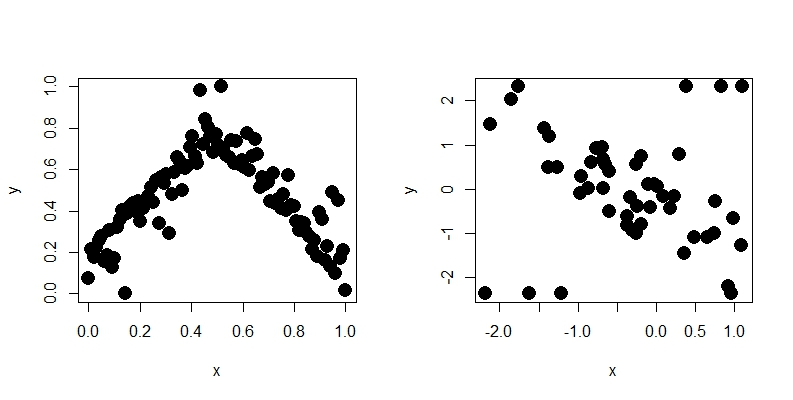
\includegraphics[width=1\linewidth]{ch-intro/figures/me}
		\caption[Simple visual analysis in the bivariate case.]{Simple visual 
		analysis in the bivariate case. The data exhibits a strong visual 
		dependency but fails common numerical tests of dependence 
		(Table~\ref{tab:intro:me}). \textit{Left}: Dataset 1 
		(Appendix~\ref{sec:appendicies:me1plot}), \textit{Right}: Dataset 2 
		(Appendix~\ref{sec:appendicies:me2plot})}
		\label{fig:intro:meplot}
	\end{center}
\end{figure}

It is interesting to note that Dataset 2 (Figure~\ref{fig:intro:meplot}, right)
is clearly linear yet common tests of linear correlation (linear regression,
Pearson's correlation) are not significantly different from zero 
(Table~\ref{tab:intro:me}). Indeed, the data used
in these examples was purposefully constructed to be dependent but bypass common
tests for dependency. However, if it is possible to construct bivariate data 
sets in that evade common numerical methods, it is believable that
it is even easier to construct analogous data sets in higher dimensions. Hence,
no such standards of ``clean analysis'' currently exist in data science despite
its importance in financial decisions, judicial evidence, government policy, and
scientific discovery. Verification of numerical tests of dependence is 
especially important in finance as equity markets are large and involve 
billions of dollars. For instance, portfolio selection often involves 
determining the relationship among as many stocks as possible in order to 
thoroughly construct the best possible portfolio.